\documentclass[a4paper]{oblivoir}
\author{Moon Il-chul \\ \href{mailto:icmoon@kaist.ac.kr}{icmoon@kaist.ac.kr} 
   \and Ryu Jae-hyeon
 \\ \href{mailto:ljh4773@kaist.ac.kr}{ljh4773@kaist.ac.kr} }
\setcounter{chapter}{9}
\title{Chapter 9. 은닉 마르코프 모델}
\usepackage{indentfirst}
\usepackage{graphicx}
\graphicspath{ {Figure/} }
\usepackage{hyperref}
\usepackage{amsmath}
\usepackage{amssymb}
\usepackage{amsfonts}
\usepackage{dsfont}
\usepackage[]{algorithm2e}
\usepackage{chngcntr}
\counterwithin{figure}{chapter}
\setcounter{tocdepth}{2}
\setcounter{secnumdepth}{3}
\hypersetup{pdfborder={0 0 0}}
\renewcommand{\thefigure}{\thechapter-\arabic{figure}}
\renewcommand{\theequation}{\thechapter.\arabic{equation}}
\newlength\myindent
\setlength\myindent{5em}

\begin{document}
\maketitle
\tableofcontents

%\chapter{}
%-----------------------------------------------------------------
\section{은닉 마르코프 모델}
%-----------------------------------------------------------------

%-----------------------------------------------------------------
\subsection{은닉 마르코프 모델}
%-----------------------------------------------------------------

%슬라이드 1, 2, 3, 4
우리는 Chapter 8에서 k-평균 군집화와 가우시안 혼합 모델을 다뤘다. 이러한 군집화 모델에서는 2차원 또는 그 이상의 다차원 공간에 여러 점들이 나와 있을 때 그것들의 알맞은 군집을 찾아주었다. 은닉 마르코프 모델은 기존의 공간이라는 개념에 더해 시간이라는 개념을 추가로 반영한 그래프 모델이다. 다만 단순히 공간의 차원을 추가하는 것처럼 시간을 추가할 수 없다. 왜냐하면 공간은 자유자재로 변할 수 있으나 시간은 한 번 흘러가면 끝이기 때문이다. 이러한 공간과는 다른 시간이 가지는 성질을 비가역적 성질이라고 한다. Chapter 9에서는 은닉 마르코프 모델이 시간이라는 요소를 어떻게 자율 학습 모델에 반영하는지, 은닉 마르코프 모델을 적용해서 어떻게 추론을 할 수 있는지를 살펴볼 것이다. \\

은닉 마르코프 모델을 이해하기 위해서는 시계열 데이터에 대한 이해가 있어야 한다. 시계열 데이터(Time Series Data)는 시간에 따라서 변하는 데이터의 추세를 나타내며, 대표적인 예시를 주식시장이나 텍스트 마이닝(Text Mining) 등에서 찾을 수 있다. \\

\begin{figure}[ht] \centering 
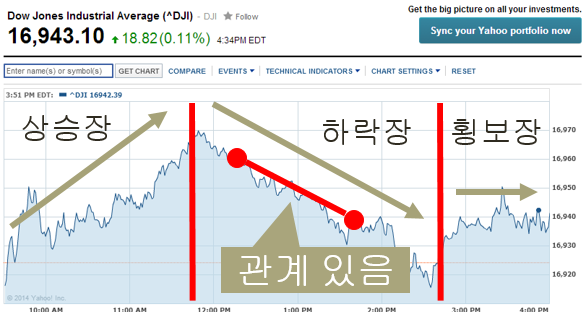
\includegraphics[scale=1.0]{fig9_1.png} 
\caption{주가지수의 변동}
\label{fig:9-1}
\end{figure}

먼저 시계열 데이터의 대표적인 예시로는 시간에 따른 주가지수의 변동이 있다. 그림 \ref{fig:9-1}은 다우 존스 산업평균지수가 시간에 따라서 어떻게 변하는지를 나타낸다. 이에 따르면 이 날의 주가지수는 주식시장이 개시하면서 상승하다가 12시부터는 반대로 하락하기 시작해서 3시까지 계속 하락하며 3시부터는 대체로 일정 수준으로 유지된다. 만일 새로운 정보가 없다면 주가지수의 변화는 일정하게 나타나며, 특정 구간 내에 잠재 변수가 있어 구간의 변화 수준을 결정한다고 생각할 수 있다. 또한 새로운 정보가 시장에 들어온다면 상승장이 하락장으로 바뀌거나 하락장이 횡보장으로 바뀌는 등의 변화가 생긴다. 이 때, 새로운 정보가 무엇인지 관찰하지 못하더라도 주가를 결정하는 잠재적인 요소에 변화가 있었다고 추측할 수 있다. 두 경우 모두 이전의 주가 변동이 이후의 주가 변동에 영향을 미치게 되며, 시간 변화를 반영하는 분석이 필요하다고 말할 수 있다. \\

\begin{figure}[ht] \centering 
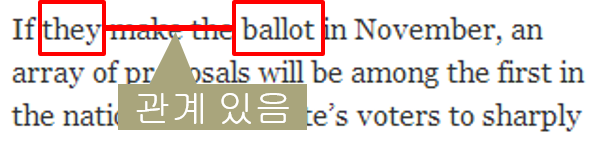
\includegraphics[scale=0.8]{fig9_2.png} 
\caption{텍스트 마이닝}
\label{fig:9-2}
\end{figure}

또 하나의 예시로는 텍스트 마이닝에서의 형태소 분석이 있다. 형태소 분석(Morphological Analysis)은 글의 단어를 주어, 동사, 목적어와 같은 품사와 어근, 접두사, 접미사 등등의 형태소로 분류하고 글을 체계적으로 분석해서 글 전체의 내용을 파악하는 것이다. 예를 들어, 화자가 그림 \ref{fig:9-2}처럼 "if they make the ballot..."라고 말했다면 분석자는 먼저 단어를 형태소에 따라서 분류하고 사용 순서를 기록한다. 그리고  분석자는 화자의 발언에는 겉으로는 확인할 수 없는 의도가 있다고 추측하고 나름의 분석을 통해서 의도를 찾는다. 여기서는 ballot이라는 목적어가 they라는 주어 뒤에 쓰였기 때문에 두 단어 사이에 관계가 있다고 추측할 수 있으며, 더 나아가 they라는 주어 뒤에 ballot이라는 목적어를 사용하도록 만든 잠재적인 요소를 찾을 수 있다.  \\

\begin{figure}[ht] \centering 
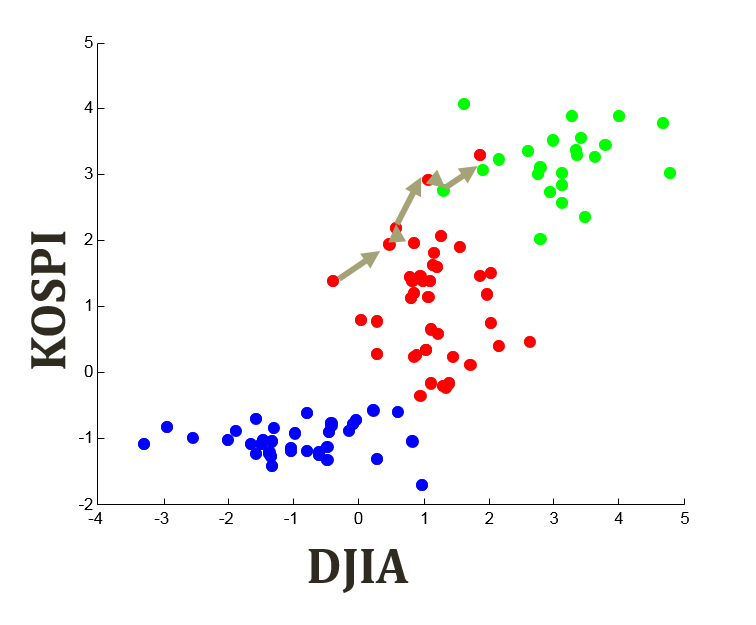
\includegraphics[scale=0.8]{fig9_3.png} 
\caption{군집화 모델}
\label{fig:9-3}
\end{figure}

주식시장으로 다시 돌아와서 이번에는 코스피 지수(KOSPI)와 다우 존스 산업평균지수(DJIA)를 그림 \ref{fig:9-3}의 그래프로 나타내 보았다. 이것을 시계열 데이터의 비가역성을 고려하지 않고 군집화를 한다면 파란색의 하락장, 빨간색의 횡보장, 그리고 초록색의 상승장으로 군집화를 할 수 있다. 그러나 이것들이 시계열 데이터라는 사실을 생각한다면 각각의 점들이 어떤 순서로 변하는지를 추가로 고려해야 한다. 예를 들어, 중앙의 빨간색 점은 시간 흐름에 따라서 위치가 변하면서 잠재 정보 또한 빨간색에서 초록색으로 바뀐다. 따라서 일반적인 군집화에서의 k-평균 군집화나 가우시안 혼합 모델을 그대로 적용한다면 시계열 데이터의 특성을 무시한 채로 분석을 진행한 것이 되어 정확한 분석이라고 할 수 없다. 따라서 시계열 데이터를 분석하기 위해서 기존의 군집화 모델을 개선할 필요가 있다. \\

%슬라이드 5
\begin{figure}[ht] \centering 
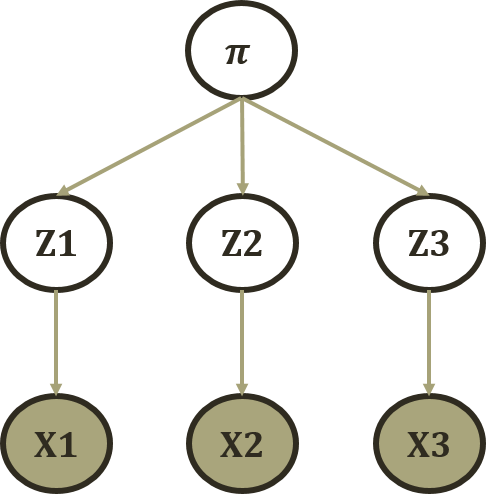
\includegraphics[scale=0.6]{fig9_4.png} 
\caption{시간 관계를 고려하지 않은 그래프 모델}
\label{fig:9-4}
\end{figure}

그림 \ref{fig:9-4}의 그래프 모델에서는 파라미터 $\pi$만이 잠재 변수 $Z_i$에 영향을 주며, 이와 달리 다른 잠재 변수들은 영향을 주지 않는다. 따라서 우리가 지금까지 배운 시간의 흐름을 반영하지 않는 그래프 모델에서는 각각의 데이터 포인트가 서로 독립이다. \\

\begin{figure}[ht] \centering 
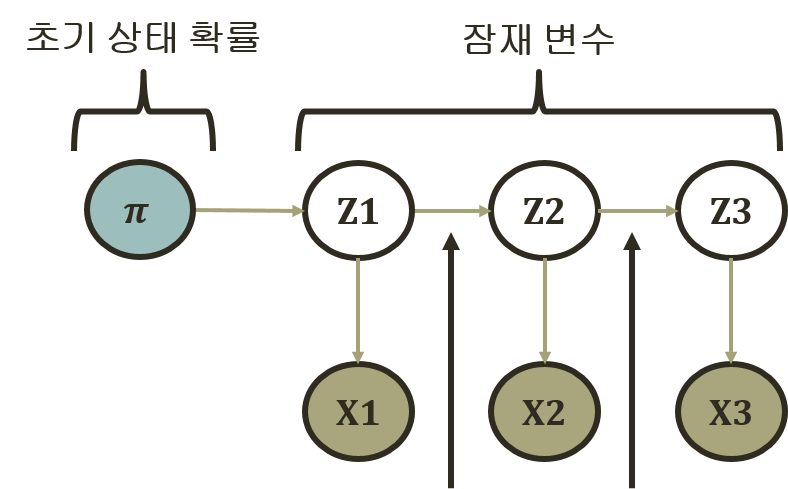
\includegraphics[scale=0.6]{fig9_5.png} 
\caption{시간 관계를 고려한 그래프 모델}
\label{fig:9-5}
\end{figure}

%슬라이드 6-1
이제는 시간의 흐름을 모델에 반영하도록 하겠다. 모델에 초기 상태 확률인 파라미터 $\pi$가 주어져 있는 것은 이전과 같다. 그러나 이번에는 잠재 변수가 다음 시점의 잠재 변수에 영향을 준다고 가정하겠다. 이렇게 한다면 시간의 흐름에 따라서 변화하는 보이지 않는 잠재 요소를 모델에 반영할 수 있다. 예를 들어, $Z_1$이 $Z_2$보다, $Z_2$가 $Z_3$보다 먼저 나타난다면 $Z_1$이 $Z_2$에, $Z_2$가 $Z_3$에 영향을 미친다고 생각할 수 있는 것이다. 이러한 시간 관계(Temporal Relation)를 반영한 모델을 그림 \ref{fig:9-5}와 같은 그래프 모델로 나타낼 수 있다.  \\

\begin{figure}[ht] \centering 
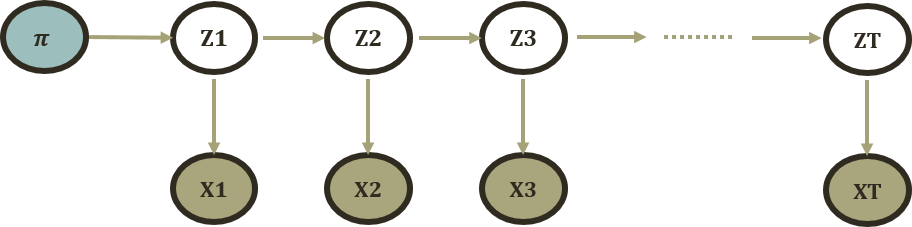
\includegraphics[scale=0.7]{fig9_6.png} 
\caption{은닉 마르코프 모델}
\label{fig:9-6}
\end{figure}

아까와 같은 식으로 시간 관계를 반영한 군집화를 동적 군집화(Dynamic Clusturing)라고 한다. 그리고 동적 군집화에서도 특별히 가우시안 혼합 모델에 시간에 따른 인과 관계를 반영한 것을 은닉 마르코프 모델(Hidden Markov Model)이라고 한다. 은닉 마르코프 모델을 그래프 모형으로 나타내면 그림 \ref{fig:9-6}과 같으며, 여기에는 시간 $1$부터 시간 $T$까지의 정수값을 가지는 시간의 흐름이 반영되어 있다. 또한, 각각의 시간 $t$에 대해서 우리가 관측할 수 있는 데이터를 뜻하는 관측 변수 $X_t$와 겉으로 드러나지 않는 잠재 변수 $Z_t$가 있다. 여기서 서로 다른 관측 변수 사이에는 시간의 흐름에 따른 연관 관계가 있지만 이것의 직접적인 원인은 어디까지나 시간의 흐름에 따른 잠재 변수의 변화에 있다. 예를 들어, $X_1$과 $X_2$는 같은 군집에 있지만 $X_3$는 다른 군집에 있다면, 이것은 잠재 변수가 $Z_1$에서 $Z_2$로 넘어갈 때에는 변화가 없었지만 $Z_2$에서 $Z_3$로 넘어가면서 군집에 변화가 있었고 그것이 $X_3$에 반영되었다는 의미이다. \\

우리는 은닉 마르코프 모델 또한 가우시안 혼합 모델처럼 $K$개의 군집이 있어서 $K$개의 가우스 분포로부터 각 데이터 포인트의 분포가 나온다는 것을 알 수 있다. 차이가 있다면 시간에 따른 인과 관계가 추가되었을 뿐이다. 또 다른 차이로는 은닉 마르코프 모델에는 잠재 변수가 각각의 데이터 포인트가 속한 군집을 나타내는 이산적인 경우로부터 한 발짝 더 나아가 연속인 경우까지 다룰 수 있다는 점이다. 이렇게 잠재 변수 $Z_t$가 연속 확률 변수일 경우의 은닉 마르코프 모델을 칼만 필터(Kalman Filter)라고 한다. 다만 여기서는 군집화의 관점에서 잠재 변수가 이산 확률 변수인 경우만을 다루도록 하겠다. \\

%슬라이드 6-2
지금까지의 설명을 수식으로 한번 나타내어 보겠다. 먼저, 맨 처음 잠재 변수인 $Z_1$은 파라미터로 $\pi_1,\cdots,\pi_k$를 가지는 다항 분포를 따른다. 이처럼 맨 처음에 위치한 잠재 변수는 초기 상태 확률(Initial State Probabilities)을 가진다. 다음으로, 잠재 변수에서 잠재 변수로 넘어가는 경우를 생각해야 한다. 여기서 잠재 변수란 데이터 포인트가 어떤 군집에 속할지를 의미하므로, 여기서는 특정 군집에서 다른 군집으로 넘어갈 확률을 생각해주어여 한다. 시간 $t$에서 $i$번째 군집에 속할 때 다음 시점인 시간 $t+1$에서 $j$번째 군집에 속할 확률을 $a_{i,j}$로 표현하겠다. 이러한 확률을 전이 확률(Transition Probability)이라고 하며, 수식으로 나타내면 다음과 같다. 
\begin{equation}
a_{i,j} = P(Z_{t+1}^j=1|Z_{t}^i=1)
\label{eq:9-1}
\end{equation}
마지막으로, 잠재 변수에서 관측 변수로 넘어가는 경우에 대해서 생각해야 한다. 관측 변수 $X_t$는 그것이 속한 군집을 의미하는 $Z_t$에 따라서 분포가 결정된다. 여기서 $X_t$ 또한 다항 분포를 가진다고 가정하면 $i$번째 군집에 속하는 데이터 포인트가 $j$로 나타날 확률을 $b_{i,j}$로 표현하겠다. 이러한 확률을 출력 확률(Emission Probaiblity)이라고 하며, 수식으로는 다음과 같이 나타낼 수 있다.     
\begin{equation}
b_{i,j} = P(X_{t}^j=1|Z_{t}^i=1)
\label{eq:9-2}
\end{equation}
따라서 은닉 마르코프 모델에서 우리가 자율 학습으로 알아야 할 파라미터에는 초기 상태 확률의 $\pi$, 전이 확률의 $a$, 그리고 출력 확률의 $b$가 있다. \\

\begin{figure}[ht] \centering 
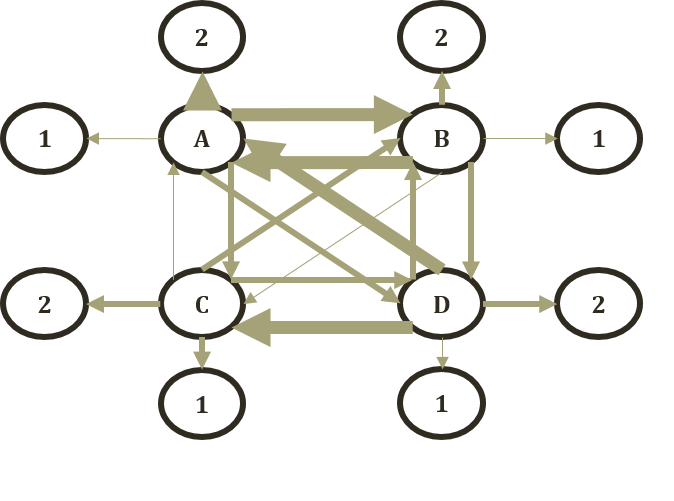
\includegraphics[scale=0.7]{fig9_7.png} 
\caption{전이 확률과 출력 확률}
\label{fig:9-7}
\end{figure}

그림 \ref{fig:9-7}의 그래프 모델은 은닉 마르코프 모델의 전이 확률과 출력 확률을 나타내며 화살표의 굵기에 따라서 확률값이 얼마나 많고 적은지를 알 수 있다. 이 그래프 모델에서 잠재 변수의 가능한 상태에는 $A$, $B$, $C$, 그리고 $D$가 있으며, 관찰 변수의 가능한 상태에는 $1$과 $2$가 있다. 여기서 특정 데이터 포인트는 시간의 흐름에 따라서 상태가 변한다. 이것은 이전의 잠재 변수의 상태에 따라서 지금의 잠재 변수의 상태가 변한 채로 나타나며, 잠재 변수 상태에 따라서 관찰 변수의 상태 또한 변한다는 것이다. 예를 들어, $A$를 기쁨, $B$를 화남, $C$를 슬픔, $D$를 즐거움이라고 하고 $1$을 좋은 표정, $2$를 나쁜 표정이라고 하자. 그러면 시간에 따라서 감정 상태가 변하며, 그에 따라서 겉으로 드러나는 표정 또한 변한다는 것으로 은닉 마르코프 모델을 비유적으로 설명할 수 있다. 이렇게 시간에 따라서 잠재 변수가 변하고 거기서 표출되는 우리의 관찰 또한 변한다는 것이 은닉 마르코프 모델의 특징이다. \\

%-----------------------------------------------------------------
\subsection{은닉 마르코프 모델에서의 확률 계산}
%-----------------------------------------------------------------

%슬라이드 7
이제는 지금까지 설명한 은닉 마르코프 모델에서 어떻게 확률값을 계산할 수 있을지를 알아보도록 하겠다. 이를 위해서 은닉 마르코프 모델의 그래프 구조 $M$이 주어졌을 때 어떤 유형의 질문을 할 수 있는지를 우선 확인해야 한다. 먼저 파라미터 $\pi$, $a$, $b$와 관찰 변수인 $X$의 값이 주어졌을 때 실제로 $X$가 관찰한 값대로 나올 확률을 알아보는 평가 질문(Evaluation Question)이 있다. 평가 질문을 수식의 형태로 나타내면 다음과 같다.
\begin{equation}
\textrm{Prob} = P(X|M, \pi, a, b)
\label{eq:9-3}
\end{equation}
다음에는 파라미터 $\pi$, $a$, $b$와 관찰 변수인 $X$의 값이 주어졌을 때 가장 알맞은 잠재 변수의 값을 알아보는 복호 질문(Decoding Question)이 있다. 복호 질문을 수식의 형태로 나타내면 다음과 같다. 
\begin{equation}
z^{*} = \textrm{argmax}_{z} P(Z=z|M, \pi, a, b, X)
\label{eq:9-4}
\end{equation}
마지막은 매우 어려우면서도 기계 학습의 본질에 가장 가까운 질문으로서 파라미터의 값을 모르는 상태에서 관찰로 주어진 $X$의 값이 실제로 나올 확률을 최대화하는 파라미터 $\pi$, $a$, $b$를 찾는 학습 질문(Learning Question)이 있다. 여기서 우리는 파라미터와 은닉 변수 양쪽 모두를 알지 못하기 때문에 학습 질문에 제대로 답하기 위해서는 가우시안 혼합 모델에서처럼 EM 알고리즘을 적절히 활용할 필요가 있다. 학습 질문을 수식의 형태로 나타내면 다음과 같다. 
\begin{equation}
(\pi^{*}, a^{*}, b^{*}) = \textrm{argmax}_{\pi, a, b} P(X|M, \pi, a, b)
\label{eq:9-5}
\end{equation}
여기서 복호 질문, 학습 질문은 각각 지도 학습, 자율 학습과 상당히 유사하다고 할 수 있다. 복호 질문에서는 파라미터가 모두 정해진 상황에서 관찰 변수가 주어졌을 때 잠재 변수를 찾는다는 의미에서 지도 학습의 성격을 지닌다. 한편, 학습 질문에서는 파라미터가 정해지지 않은 상황에서 동적 군집화를 적용해서 적절한 파라미터를 적용하므로 자율 학습의 성격을 지닌다. 그러나 어떤 확률을 구하든지 간에 계산에 필요한 파라미터에 대해서 충분히 이해하고 있어야만 이러한 질문들에 답을 내릴 수 있다. \\  

%슬라이드 8
그렇다면 은닉 마르코프 모델의 그래프 구조 $M$과 관찰 변수 $X$의 값이 주어졌을 때 파라미터의 값을 어떻게 구할 수 있을까? 주사위 던지기 게임을 통해서 이것을 살펴보도록 하겠다. 주사위 던지기 게임에 참가하는 참가자는 딜러가 던지는 주사위의 숫자를 정확히 맞춰야 한다. 이 게임에서 몇몇 주사위는 무게 중심이 조금 이동해 있어서 던지면 6이 나올 확률이 1/6보다 높다고 하며 이러한 주사위를 속임수 주사위(Loaded Dice, L)라고 하겠다. 반면에 주사위의 각 숫자가 나올 확률이 정확히 1/6인 주사위를 일반 주사위(Fair Dice, F)라고 하겠다. 게임에는 이러한 두 종류의 주사위를 사용하지만 어떤 주사위를 사용했는지는 오로지 딜러만이 알고 있으며 참가자는 알 수 없게 되어 있다. 딜러는 이러한 딜러와 참가자 사이의 정보 불균형을 이용해서 일반 주사위와 속임수 주사위를 자유자재로 바꿔가면서 게임을 진행한다. \\

이러한 규칙의 주사위 던지기 게임을 은닉 마르코프 모델로 놓고 생각하면 L과 F 중에서 어떤 주사위를 사용했는지를 잠재 변수로, 주사위를 던져서 어떤 숫자가 나왔는지를 관찰 변수로 볼 수 있다. 그리고 파라미터 $a_{L,L}$은 딜러가 처음에 속임수 주사위를 사용했을 때 바로 다음에도 속임수 주사위를 사용할 확률과 같으며 다른 $a$의 성분에 대해서도 같은 식으로 정할 수 있다. 파라미터 $b$에 대해서도 $b_{L,1}$은 속임수 주사위를 던졌을 때 1이 나올 확률과 같으며 다른 $b$의 성분의 값 또한 지정해 줄 수 있다. \\

\begin{figure}[ht] \centering 
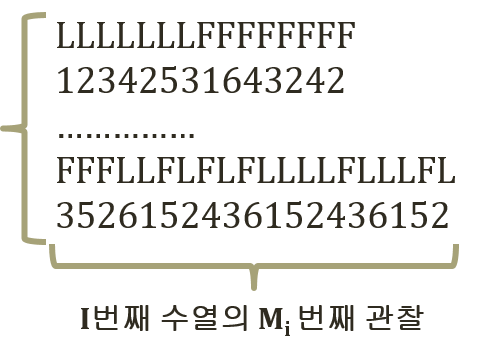
\includegraphics[scale=1.0]{fig9_8.png} 
\caption{일반 주사위(F)와 속임수 주사위(L)를 던진 결과}
\label{fig:9-8}
\end{figure}

이제 우리가 원하는 대로 파라미터 값을 어떻게 찾을지를 생각해보자. 그림 \ref{fig:9-8}과 같이 관찰 결과가 잠재 변수와 관찰 변수, 양쪽 모두에 대해서 주어져 있다면 우리는 chapter 1에서 배웠던 MLE나 MAP 또는 카운팅으로 적절한 파라미터 값을 찾을 수 있다. 예를 들어, 제일 단순한 방법인 카운팅을 적용해서 초기 상태 확률 $\pi$를 계산하려 한다면 각 수열에서 첫 번째 잠재 변수만을 골라서 L과 F의 개수를 헤아리면 된다. 그리고 전이 확률 $a$를 계산하기 위해서는 L과 F에 대해서 각각 다음에 나오는 L과 F의 개수를 헤아리면 된다. 마지막으로 출력 확률 $b$를 계산하기 위해서는 주사위를 던졌을 때 나오는 수를 L과 F의 두 가지 경우 각각에 대해서 1부터 6까지의 값을 가지는 관찰 변수를 헤아리면 된다. \\

%슬라이드 9
\begin{figure}[ht] \centering 
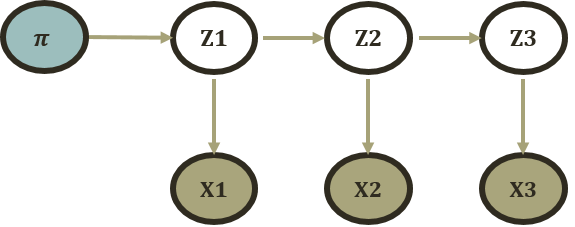
\includegraphics[scale=0.45]{fig9_9.png} 
\caption{은닉 마르코프 모델 예시}
\label{fig:9-9}
\end{figure}

은닉 마르코프 모델 또한 베이지안 네크워크의 일종이다. 따라서 베이지안 네트워크에서 다룬 것들을 활용해서 확률이나 파라미터를 계산할 수 있다. 먼저 그림 \ref{fig:9-9}와 같이 은닉 마르코프 모델의 구조와 $X$와 $Z$를 포함하는 학습 데이터가 주어져 있다고 생각하겠다. 그러면 $X$와 $Z$의 전체 결합 확률 분포 $P(X,Z)$를 다음과 같이 분해할 수 있다. 
\begin{eqnarray}
P(X,Z) & = & P(X_{1},X_{2},X_{3},Z_{1},Z_{2},Z_{3}) \nonumber \\
& = & P(Z_{1}) P(X_{1}|Z_{1}) P(Z_{2}|Z_{1}) P(X^{2}|Z_{2}) \nonumber \\ 
& & \ \ \ \ \ \ \ \ \ \ \ \ \ \ \ \ \ \ \ \ \ \ \ \ \ \ \ \ \cdot \ P(Z_{3}|Z_{2}) P(X_{3}|Z_{3}) \label{eq:9-6}
\end{eqnarray}
여기서 $P(Z_{1})$은 초기 상태 확률, $P(Z_{2}|Z_{1})$, $P(Z_{3}|Z_{2})$는 전이 확률, $P(X_{1}|Z_{1})$, $P(X_{2}|Z_{2})$, $P(X_{3}|Z_{3})$는 출력 확률에 해당된다. 이처럼 결합 확률은 초기 상태 확률과 여러 개의 전이 확률, 출력 확률의 곱으로 분해할 수 있다. 이제 결합 확률에 관찰값인 $x$, $z$와 파라미터 $\pi$, $a$, $b$를 수식 (\ref{eq:9-6})에 알맞게 대입하면 다음과 같이 나타낼 수 있다.  
\begin{equation}
P(X=x,Z=z) = {\pi}_{Z_{1}} \cdot {b}_{X_{1},Z_{1}} \cdot {a}_{Z_{1}, Z_{2}} \cdot {b}_{x_{2},Z_{2}} \cdot {a}_{Z_{2}, Z_{3}} \cdot {b}_{x_{3},Z_{3}} \label{eq:9-7} 
\end{equation} 

이제 앞에서의 다룬 주사위 던지기 게임를 다시 들고와서 결합 확률의 분해식이 맞는지를 확인하도록 하겠다. 사전에 주어진 데이터로부터 속임수 주사위(L)에서 1, 2, 3, 4, 5가 나올 확률으로 1/10이, 6이 나올 확률으로 1/2가 나왔다고 생각하자. 그리고 딜러가 처음에 속임수 주사위를 쓸 확률을 1/2, 일반 주사위를 쓴 바로 다음에 일반 주사위를 다시 쓸 확률을 1/2, 속임수 주사위를 쓴 바로 다음에 속임수 주사위를 다시 쓸 확률을 7/10이라고 가정하겠다. 여기서 주사위를 세 번 연속해서 던졌을 때 순서대로 1, 6, 6이 나왔다면 세 번 모두 일반 주사위를 썼을 확률과 세 번 모두 속임수 주사위를 썼을 확률을 비교해서 어느 쪽이 더 가능성이 높은지를 알아보려 한다. 먼저 전자의 확률은 다음과 같이 계산할 수 있다. 
\begin{eqnarray}
P(X=166,Z=LLL) & = &  {\pi}_{L} \cdot {b}_{1,L} \cdot {a}_{L,L} \cdot {b}_{6,L} \cdot {a}_{L,L} \cdot {b}_{6,L} \nonumber \\
& = & \frac{1}{2} \times \frac{1}{10} \times \frac{7}{10} \times \frac{1}{2} \times \frac{7}{10} \times \frac{1}{2} \nonumber \\
& = & 6.125 \times 10^{-3} \label{eq:9-8}
\end{eqnarray}
또한, 후자의 확률은 다음과 같이 계산할 수 있다. 
\begin{eqnarray}
P(X=166,Z=FFF) & = & {\pi}_{F} \cdot {b}_{1,F} \cdot {a}_{F,F} \cdot {b}_{6,F} \cdot {a}_{F,F} \cdot {b}_{6,F} \nonumber \\
& = & \frac{1}{2} \times \frac{1}{6} \times \frac{1}{2} \times \frac{1}{6} \times \frac{1}{2} \times \frac{1}{6} \nonumber \\
& = & 5.7870 \times 10^{-4} \label{eq:9-9}
\end{eqnarray}
세 번 모두 가짜 주사위를 썼을 확률이 약 12배 높으므로 속임수 주사위를 던졌다고 생각하는 편이 훨씬 합리적이라고 결론내릴 수가 있다. 그리고 여기서는 LLL과 FFF 외에 다른 시나리오에 대해서도 결합 확률값을 확인하는 것이 더욱 꼼꼼한 조사가 될 것이다. 그러나 모든 경우를 살펴보기 위해서는 지수적으로 많은 횟수만큼 결합 확률을 계산해야 한다. 여기서는 세 번 던졌을 뿐이므로 $2 \times 2 \times 2 = 8$번의 계산이면 된다. 그러나 주사위를 한 번씩 추가로 던질 때마다 경우의 수가 2배로 늘어나며 $N$번 던졌을 경우에는 총 $2^N$번의 계산이 필요하게 된다. 따라서 모든 경우에 대해서 결합 확률을 구하는 대신 다른 방법을 찾을 필요가 있다. \\

%슬라이드 10-1
결합 확률을 대신할 방법을 이해하기 위해서는 주변 확률에 대해서 알아야 한다. 주변 확률(Marginal Probability)은 결합 확률을 모든 잠재 변수 $Z$에 대해서 주변화한 확률이다. 가우시안 혼합 모델에서 $P(X|\theta)$를 $\sum_{Z} P(X,Z|\theta)$로 나타낸 것과 같이 은닉 마르코프 모델에서는 $P(X|\pi,a,b)$를 $\sum_{Z} P(X,Z|\pi,a,b)$로 나타낼 수 있다. 이것을 다음과 같이 풀어 쓸 수 있다.
\begin{eqnarray}
P(X|\pi,a,b) & = & \sum_{Z=z} P(X,Z|\pi,a,b) \nonumber \\
& = & \sum_{Z_{1}} \cdots \sum_{Z_{T}} P(X_{1},\cdots,X_{T},Z_{1},\cdots,Z_{T}) \nonumber \\
& = & \sum_{Z_{1}} \cdots \sum_{Z_{T}} {\pi}_{Z_{1}} \prod_{t=2}^{T} a_{Z^{t-1},Z_{T}} \prod_{t=1}^{T} b_{Z_{T},X_{t}} \label{eq:9-10}
\end{eqnarray}
그러나 이 또한 계산하기에 쉬운 방법은 아니라고 할 수 있다. 우리는 다음 내용에서 설명할 재귀 개념을 이용하고 있는 전향-후향 확률 계산 알고리즘으로 결합 확률값을 구해서 평가 질문에서 답하고자 한다. \\

%-----------------------------------------------------------------
\subsection{전향-후향 확률 계산}
%-----------------------------------------------------------------

%슬라이드 11, 12
전향-후향 확률 계산이 무엇인지를 알기 위해서는 먼저 재귀를 이해하고 있어야 한다. 여기서 재귀(Recursive)란 하나의 큰 문제를 여러 개의 작은 부문제로 나누어서 해결하는 분할 정복 알고리즘(Divide and Conquer Algorithm)이다. 재귀를 정의하기 위해서는 함수를 정의할 때 자기 자신을 그대로 참조하는 재귀 함수(Recursive Function)를 사용한다. 이러한 재귀 함수는 초기 상태의 값을 지정한 초기값과 재귀 함수 자신을 포함하는 재귀식으로 이루어져 있다. \\

\begin{figure}[ht] \centering 
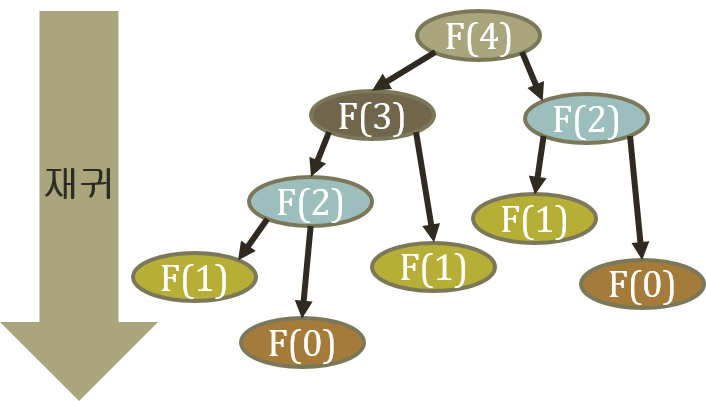
\includegraphics[scale=0.6]{fig9_10.png} 
\caption{재귀를 사용한 피보나치 수열 계산}
\label{fig:9-10}
\end{figure}

재귀로 구할 수 있는 대표적인 예시에는 피보나치 수가 있다. 피보나치 수는 바로 앞에 있는 두 피보나치 수의 합으로 정의할 수 있다. $n$번째 피보나치 수를 $F(n)$이라고 하면 우리는 재귀 함수의 초기값을 $F(0)=1$, $F(1)=1$, 재귀식을 $F(n) = F(n-1) + F(n-2)$으로 구성할 수 있다.  그러면 그림 \ref{fig:9-10}에서처럼 $F(4)$를 계산하기 위해서 이것을 $F(3)$과 $F(2)$로 분할한다. 그리고 $F(3)$과 $F(2)$를 계산하기 위해서 이것들을 각각 $F(2)$와 $F(1)$, $F(1)$과 $F(0)$으로 나누게 된다. 여기서 $F(1)$과 $F(0)$은 그 값이 각각 1과 0으로 지정되어 있으므로 이것들을 모두 더해서 $F(2)=2$를 구할 수 있다. 이런 식으로 이미 값이 지정된 $F(1)$와 $F(0)$이 나올 때까지 문제를 계속해서 분할해서 처리하는 방법이 바로 재귀이다. 이처럼 재귀는 맨 꼭대기에서부터 시작해서 문제를 여러 개의 부문제로 분할하면서 아래로 내려가는 하향식 접근(Top Down Approach)을 따른다.\\

\begin{figure}[ht] \centering 
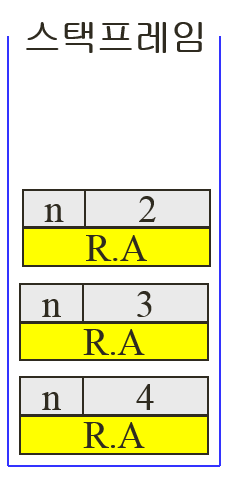
\includegraphics[scale=0.6]{fig9_11.png} 
\caption{스택프레임}
\label{fig:9-11}
\end{figure}

재귀를 효율적으로 프로그래밍하기 위해서 사용한 것으로 스택프레임(Stackframe)이 있다. 스택프레임은 나중에 들어온 것이 먼저 나가는 LIFO(Last In, First Out) 원칙을 따르는 자료 구조인 스택을 도입한 것이다. 피보나치 수열의 계산에 있어서 $F(4)$를 계산하기 위해서는 먼저 $F(4)$를 스택프레임에 넣는다. 다음으로 $F(4)$를 계산하기 위해서 필요한 $F(3)$과 $F(2)$를 스택프레임에 넣는다. 그 이후에도 재귀의 순서에 따라서 재귀 함수를 넣고 빼기를 반복하며 마지막에는 맨 처음에 들어간 $F(4)$가 나오면서 전체 과정이 끝난다. 여기서 스택프레임은 나중에 들어온 $F(3)$과 $F(2)$를 먼저 계산한 뒤 이들을 더해서 마지막으로 $F(4)$를 계산한다. \\

재귀 알고리즘은 큰 문제를 여러 개의 작은 문제로 나누어서 해결하는 강력한 방법이다. 그러나 여기에는 한 가지 문제가 있다. 위에서 4번째 피보나치 수인 $F(4)$를 계산하기 위해서 $F(3)$을 1번, $F(2)$를 2번 계산하였다. 여기서 $F(2)$의 사용은 $F(4)$를 계산하기 위해서 한 번, $F(3)$을 계산하기 위해서 다시 한 번 이루어졌다. 이와 같이 재귀에서는 큰 문제를 여러 개의 작은 부문제로 분할해서 해결하는데, 이 때 동일한 내용의 부문제를 여러 번 계산할 수 있다. 그 때문에 문제가 크면 클수록 반복해서 계산할 것이 많아지게 된다. 따라서 문제의 규모가 크면 클수록 재귀를 사용해서 문제를 풀기는 더욱 어려워진다. \\

동적 계획법(Dynamic Programming)은 재귀에서 같은 부문제를 여러 번 풀어야 한다는 비효율적인 부분을 개선한 방법이다. 동적 계획법에서는 처음 한 번은 부문제를 풀어서 그 결과를 메모이제이션 표(Memoization Table)에 저장한다. 그러면 이후에 다시 부문제를 풀어야 할 때 기존의 계산을 반복하는 대신에 메모이제이션 표에서 이전에 저장한 값을 그대로 가져오는 식으로 문제 해결을 진행한다. 다시 말해서 동적 계획법은 이전에 해결한 부문제의 해답을 재활용해서 큰 문제의 해답을 계산하는 것이 된다. \\

\begin{figure}[ht] \centering 
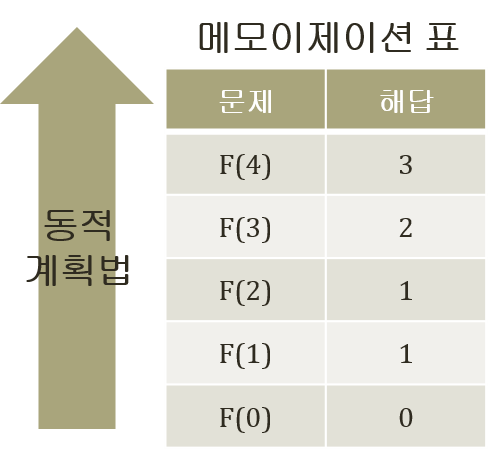
\includegraphics[scale=0.6]{fig9_12.png} 
\caption{메모이제이션 표}
\label{fig:9-12}
\end{figure}

예를 들어, 이번에는 동적 계획법을 활용해서 4번째 피보나치 수를 계산하겠다. 맨 처음에는 주어진 초기값인 $F(0)=0$, $F(1)=1$을 메모이제이션 표에 저장한다. 다음으로 $F(0)$과 $F(1)$을 더해서 $F(2)=1$를 계산하고 이를 메모이제이션 표에 저장한다. 같은 식으로 $F(3)=2$와 $F(4)=3$을 계산해서 메모이제이션 표에 마찬가지로 저장한다. 이 때, 우리가 주목해야 할 것은 $F(4)$를 계산하기 위해서는 $F(3)$과 $F(2)$의 값이 필요한데 이것을 직접 계산하는 대신에 메모이제이션 표에서 이전에 저장한 $F(3)$과 $F(2)$의 값을 가져왔다는 것이다. 그 덕분에 $F(3)$과 $F(2)$를 따로 계산할 필요가 없게 된다. 이처럼 동적 계획법은 작은 문제의 답에서부터 시작해서 큰 문제의 답을 메모이제이션 표에 점차 채워나가는 상향식 접근(Bottom Up Approach)을 따른다.

%슬라이드 10-2
\begin{figure}[ht] \centering 
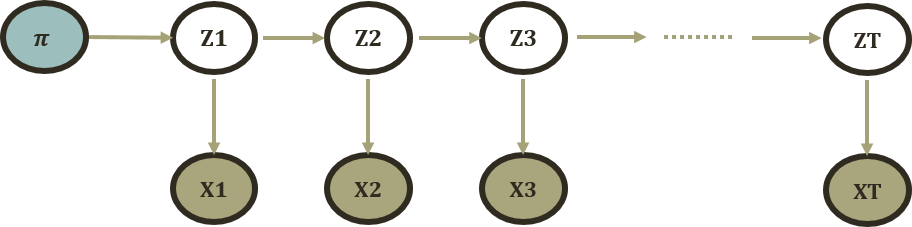
\includegraphics[scale=0.7]{fig9_6.png} 
\caption{은닉 마르코프 모델}
\label{fig:9-13}
\end{figure}

재귀와 동적 계획법을 활용해서 이제는 결합 확률을 계산할 수 있는 방법을 설명할 수 있게 되었다. 먼저 원래의 은닉 마르코프 모델에서 임의의  $t$에 대해서 $X_{1},\cdots,X_{t}$와 $Z_{t}$, $Z_{t-1}$만을 가지는 축소된 그래프 모델을 생각하겠다. 그리고 $X_{1},\cdots,X_{t}$와 $Z_{t}$만을 가지는 결합 확률의 값을 주변화 과정을 통해서 전개해서 나타내어 보겠다. 
\begin{eqnarray}
P(X_{1},\cdots,X_{t},Z_{t}) & = & \sum_{Z_{t-1}} P(X_{1},\cdots,X_{t-1},X_{t},Z_{t-1},Z_{t}) \nonumber \\
& = & \sum_{Z_{t-1}} P(X_{1},\cdots,X_{t-1},Z_{t-1}) P(X_{t},Z_{t}|X_{1},\cdots,X_{t-1},Z_{t-1})  \nonumber \\
& = & \sum_{Z_{t-1}} P(X_{1},\cdots,X_{t-1},Z_{t-1}) P(Z_{t}|X_{1},\cdots,X_{t-1},Z_{t-1}) \nonumber \\ 
&  &  \ \ \ \ \ \ \ \ \ \ \cdot \ P(X_{t} | X_{1},\cdots,X_{t-1},Z_{t-1},Z_{t})  \label{eq:9-11}
\end{eqnarray}
여기에 그림 \ref{fig:9-13}의 그래프 구조를 활용해서 수식 (\ref{eq:9-11})을 다음과 같이 나타낼 수 있다. 
\begin{eqnarray}
P(X_{1},\cdots,X_{t},Z_{t}) & = & \sum_{Z_{t-1}} P(X_{1},\cdots,X_{t-1},Z_{t-1}) P(Z_{t}|Z_{t-1}) P(X_{t} | Z_{t}) \nonumber \\ 
& = & \sum_{Z_{t-1}} P(X_{1},\cdots,X_{t-1},Z_{t-1}) a_{Z_{t-1},z_{t}} b_{Z_{t},X_{t}} \nonumber \\
& = & b_{Z_{t},X_{t}} \sum_{Z_{t-1}} a_{Z_{t-1},z_{t}} P(X_{1},\cdots,X_{t-1},Z_{t-1}) \label{eq:9-12}
\end{eqnarray}
지금까지의 전개에서 나타난 $P(X_{1},\cdots,X_{t-1},Z_{t-1})$은 $P(X_{1},\cdots,X_{t},Z_{t})$의 $t$를 하나 줄어든 값인 $t-1$로 바꾼 것과 같다. 또한, 모든 가능한 $Z_{t-1}$에 대해서, 다시 말해 $X_{t-1}$이 포함될 수 있는 모든 군집에 대해서, $P(X_{1},\cdots,X_{t-1},Z_{t-1})$의 값을 알고 있으면 $P(X_{1},\cdots,X_{t},Z_{t})$을 계산할 수 있다. 따라서 수식 (\ref{eq:9-12})는 $P(X_{1},\cdots,X_{t},Z_{t})$의 재귀식이 될 수 있다. \\

%슬라이드 13
이것을 이제 재귀 함수로 나타내어 보겠다. 먼저 $Z_{t}^{k}=1$을 시간 $t$에서의 데이터 포인트가 $k$번째 클러스터에 할당된 것을 의미한다고 하겠다. 그리고 $P(X_{1},\cdots,X_{t},Z_{t}^{k}=1)$을 $\alpha_{t}^{k}$로 나타내어 보겠다. 이러한 $\alpha_{t}^{k}$를 전향 확률(Forward Probability)이라고 한다. 그러면 $\alpha_{t}^{k}$의 초기값은 각 $k$에 대해서 $t=1$일 때의 $\alpha_{t}^{k}$의 값이 된다. 이것을 다음과 같이 나타낼 수 있다. 
\begin{eqnarray}
\alpha_{1}^{k} & = & P(X_{1},Z_{1}^{k}=1) \nonumber \\
& = &  P(X_{1}|Z_{1}^{k}=1) P(Z_{1}^{k}=1) \nonumber \\
& = &  b_{k,X_{1}} \pi_{k}  \label{eq:9-13} 
\end{eqnarray}
또한, $t=2$에서부터 $t=T$까지의 경우에 대해서 각 $k$에 대한 재귀식을 다음과 같이 세울 수 있다. 
\begin{eqnarray}
\alpha_{t}^{k} & = & P(X_{1},\cdots,X_{t},Z_{t}^{k}=1) \nonumber \\
& = &  b_{k,X_{t}} \sum_{Z_{t-1}} a_{Z_{t-1},k} P(X_{1},\cdots,X_{t-1},Z_{t-1}) \nonumber \\
& = &  b_{k,X_{t}} \sum_{i} a_{i,k} \alpha_{t-1}^{i}  \label{eq:9-14} 
\end{eqnarray}
전향 확률 계산(Forward Probability Calculation)은 전향 확률에 대한 초기값과 재귀식을 활용해서 각 $t$와 $k$에 대한 $\alpha_{t}^{k}$ 값을 구하는 것이다. 여기에는 먼저 $t=1$에서 각 $k$에 대한 $\alpha_{t}^{k}$의 값인 초기값이 수식 (\ref{eq:9-13})과 같이 주어져 있다. 그러면 $t=1$일 때의 $\alpha_{t}^{k}$의 값을 활용해서 $t=2$일때의 각 $k$에 대한 $\alpha_{t}^{k}$을 구할 수 있다. 그리고 $t=2$일 때의 $\alpha_{t}^{k}$의 값을 활용해서 $t=3$일때의 $\alpha_{t}^{k}$을 구할 수 있다. 같은 식으로 이것을 $t=T$일 때까지 반복한다. 그러면 모든 $t$와 $k$에 대한 $\alpha_{t}^{k}$의 값을 구할 수 있다. 이것을 동적 계획법으로 구현하기 위해서는 $\alpha_{t}^{k}$의 값을 저장하는 메모이제이션 표를 구성해서 $\alpha_{t}^{k}$의 값을 저장해 두어야 한다. 이 때, 메모이제이션 표는 $t$가 하나씩 커질 때마다 크기가 점차 커지게 된다. \\ 

메모이제이션 표를 다 채웠으면 평가 질문에 답하기 위해서 필요한 $P(X_{1},\cdots,X_{T})$ 값을 다음과 같이 구할 수 있다. 
\begin{eqnarray}
P(X_{1},\cdots,X_{T}) & = & \sum_{Z_{T}} P(X_{1},\cdots,X_{T},Z_{T})  \nonumber \\
& = & \sum_{k} \alpha_{T}^{k} \label{eq:9-15} 
\end{eqnarray}
그러나 여기에는 한 가지 문제가 있다. $\alpha_{t}^{k}$는 시간 $t$까지의 경우만을 생각하는 확률값이다. 그러나 잠재 변수가 잠재 변수가 나온 시점까지의 관찰 변수로부터만 영향을 받는다고 생각할 수는 없다. 잠재 변수가 나온 시점 이후의 관찰 변수라도 잠재 변수와 관련이 있을 수 있는 것이다. 이런 관점으로 보면 특정 시점의 잠재 변수는 모든 시점의 관찰 변수로부터 영향을 받는다는 것을 모델에 반영해야 한다는 사실을 알 수 있다. 그런데 전방 확률은 잠재 변수가 나온 시점까지의 관찰 변수만을 반영할 수 있으므로 이후의 관찰 변수까지 반영할 수 있는 새로운 방법을 생각해야 한다. \\

%슬라이드 14
앞에서 설명한 내용을 확률 계산에 반영하기 위해서는 결합 확률을 수식 (\ref{eq:9-11})과는 다른 방법으로 나타낼 필요가 있다. 수식 (\ref{eq:9-11})에서는 결합 확률이 고려하는 관찰 변수가 $X_{1}$에서 $X_{t}$까지였다면 이번에는 이것을 $X_{T}$까지로 확장하겠다. 그러면 잠재 변수 $Z_{t}$는 $X_{1},\cdots,X_{t}$의 중간 위치에 들어가게 된다. 이것을 고려해서 결합 확률 $P(X,Z_{t})$을 분해한 것이 다음과 같다. 
\begin{eqnarray}
P(X,Z_{t}^{k}=1) & = & P(X_{1},\cdots,X_{t},Z_{t}^{k}=1,X_{t+1},\cdots,X_{T}) \nonumber \\
& = &  P(X_{1},\cdots,X_{t},Z_{t}^{k}=1)P(X_{t+1},\cdots,X_{T}|X_{1},\cdots,X_{t},Z_{t}^{k}=1) \nonumber \\
& = & P(X_{1},\cdots,X_{t},Z_{t}^{k}=1)P(X_{t+1},\cdots,X_{T}|Z_{t}^{k}=1) \label{eq:9-16}
\end{eqnarray}
여기서 $P(X_{1},\cdots,X_{t},Z_{t}^{k}=1)$는 $\alpha_{t}^{k}$와 같다. 따라서 $P(X_{t+1},\cdots,X_{T}|Z_{t}^{k}=1)$를 계산하면 된다. 우리는 $P(X_{t+1},\cdots,X_{T}|Z_{t}^{k}=1)$를 $\beta_{t}^{k}$로 정의하겠다. 이러한 $\beta_{t}^{k}$ 확률값을 후향 확률(Backward Probability)이라고 한다. 그러면 $P(X_{t+1},\cdots,X_{T}|Z_{t}^{k}=1)$에 관한 수식을 전개해서 $\beta_{t}^{k}$를 다음과 같이 나타낼 수 있다.
\begin{eqnarray}
\beta_{t}^{k} & = & P(X_{t+1},\cdots,X_{T}|Z_{t}^{k}=1) \nonumber \\
& = & \sum_{Z_{t+1}} P(X_{t+1},\cdots,X_{T}, Z_{t+1}|Z_{t}^{k}=1) \nonumber \\ 
& = & \sum_{i} P(Z_{t+1}^{i}=1|Z_{t}^{k}=1) P(X_{t+1}|Z_{t}^{k}=1, Z_{t+1}^{i}=1)  \nonumber \\
& & \ \ \ \ \ \ \ \ \ \ \ \ \ \ \ \ \ \ \ \ \ \ \ \cdot \ P(X_{t+2},\cdots,X_{T}|X_{t+1}, Z_{t}^{k}=1, Z_{t+1}^{i}=1) \nonumber \\
& = & \sum_{i} P(Z_{t+1}^{i}=1|Z_{t}^{k}=1) P(X_{t+1}|Z_{t+1}^{i}=1) P(X_{t+2},\cdots,X_{T}| Z_{t+1}^{i}=1) \nonumber \\
& = & \sum_{i} a_{k,i} b_{i,X_{t}} \beta_{t+1}^{i} \label{eq:9-17}
\end{eqnarray}
이렇게 우리는 $\beta_{t+1}^{k}$가 있으면 $\beta_{t}^{k}$의 값을 계산할 수 있다는 사실을 재귀식을 유도하여 확인하였다. 이러한 $\beta_{t}^{k}$를 후향 확률(Backward Probability)이라고 한다. 후향 확률을 계산하는데 있어 동적 계획법을 적용한다면, $\alpha_{t}^{k}$와는 정반대로 $\beta_{t}^{k}$ 값을 저장하는 메모이제이션 표는 $t=T$에서 시작해서 $t$가 하나씩 작아질 때마다 한 줄씩 채워지게 된다. 또한, 각 $k$에 대해서 $\beta_{t}^{k}$의 초기값을 다음과 같이 구할 수 있다. 
\begin{equation}
\beta_{T}^{k} = P(\ \cdot \ |Z_{t}^{k}=1) = 1
\label{eq:9-18}
\end{equation} 
이렇게 전개한 재귀식과 초기값을 활용해서 모든 $t$와 $k$에 대한 $\beta_{t}^{k}$를 계산하는 것을 후향 확률 계산(Backward Probability Calculation)이라고 한다. \\

우리는 각 $t$와 $k$에 대해서 전향 확률 계산으로 $\alpha_{t}^{k}$를, 후향 확률 계산으로 $\beta_{t}^{k}$를 계산하였다. 그러면 이제 결합 확률 $P(X,Z_{t})$을 전향 확률 $\alpha_{t}^{k}$와 후향 확률 $\beta_{t}^{k}$만으로 나타낼 수 있다. 
\begin{equation}
P(X,Z_{t}^{k}=1) = \alpha_{t}^{k} \beta_{t}^{k} 
\label{eq:9-19}
\end{equation} 
또는 재귀식인 수식 (\ref{eq:9-14})과 (\ref{eq:9-17})을 대입해서 동적 계획법의 과정에서 메모이제이션 표에 저장한 $\alpha_{t-1}^{k}$와 $\beta_{t+1}^{k}$에 관한 식으로 다음과 같이 나타낼 수 있다.  
\begin{equation}
P(X,Z_{t}^{k}=1) = (b_{k,X_{t}} \sum_{i} a_{i,k} \alpha_{t-1}^{i}) \times (\sum_{i} a_{k,i} b_{i,X_{t}} \beta_{t+1}^{i})
\label{eq:9-20}
\end{equation}  
그러면 이제는 수식 (\ref{eq:9-15})에서 했던 것처럼 특정 $t$를 하나 고르고 $P(X,Z_{t})$를 $Z_{t}$에 대해서 주변화해서 평가 질문에서 원하는 확률값을 다음과 같이 계산할 수 있다.  
\begin{eqnarray}
P(X_{1},\cdots,X_{T}) & = & \sum_{Z_{t}} P(X_{1},\cdots,X_{T},Z_{t})  \nonumber \\
& = & \sum_{k} \alpha_{t}^{k} \beta_{t}^{k} \label{eq:9-21} 
\end{eqnarray}
이렇게 우리는 전향-후향 확률 계산으로 평가 질문의 답을 내린 것이다. 전향, 후향 확률은 이후의 확률 계산 알고리즘 과정에서도 여러 차례 활용되므로 계산하는 방법과 이론적 원리를 충분히 이해할 필요가 있다.

%-----------------------------------------------------------------
\section{확률 계산 알고리즘}
%-----------------------------------------------------------------

%-----------------------------------------------------------------
\subsection{비터비 복호 알고리즘}
%-----------------------------------------------------------------

%슬라이드 19
전향-후향 확률 계산 외에도 은닉 마르코프 모델에서 확률을 분석하기 위한 여러 종류의 알고리즘이 있다. 사실 앞에서의 설명한 전향-후향 확률 계산은 평가 질문에 답을 줄 수 있다. 그러나 시계열 데이터를 포함하는 그래프 모델을 분석하는데 있어서 평가 질문의 답만 있어서는 아직 부족하다. 이제는 보다 더 강력한 질문인 복호 질문에 답하기 위한 알고리즘으로 비터비 복호 알고리즘을 제시하고자 한다. \\

우리는 앞에서 전향-후향 확률 계산으로 전향 확률 $\alpha$와 후향 확률 $\beta$에 대해서 재귀식을 세우고 동적 계획법으로 값을 구했다. 그리고 이러한 확률값들을 임의의 데이터 포인터가 특정 시점에서 특정 군집에 속할 확률을 구하는데 사용했다. 이 확률값을 각 군집별로 비교하면 각 시간별로 데이터 포인트가 속할 수 있는 가장 적절한 군집을 찾을 수 있다. 비터비 복호 알고리즘은 동적 계획법을 사용해서 데이터 포인트에 있어서 각 시간별로 가장 적절한 군집을 찾는 작업을 한 번에 수행하도록 하는 알고리즘이다. \\

비터비 복호 알고리즘을 사용하는 이유를 이해하기 위해서 복호 질문의 해답을 수식을 사용해서 나타내어 보자. 시간 $t=1,\cdots,T$에 대해서 데이터 포인트가 속하는 가장 적절한 군집 $k_{t}^{*}$는 관찰 변수의 값이 주어졌을 때 특정 군집에 속할 확률인 조건부 확률을 최대화하며, 이것을 다음과 같은 수식으로 나타낼 수 있다. 
\begin{equation}
k_{t}^{*} = \textrm{argmax}_{k} P(Z_{t}^{k} = 1 | X)
\label{eq:9-22}
\end{equation}
여기서 $P(X)$의 값이 일정하므로 조건부 확률을 최대로 만드는 것은 결합 확률을 최대로 만드는 것과 같다. 따라서 $k_{t}^{*}$를 다음과 같이 결합 확률을 사용해서 나타낼 수 있다. 
\begin{equation}
k_{t}^{*} = \textrm{argmax}_{k} P(Z_{t}^{k} = 1 | X)
\label{eq:9-23}
\end{equation}
그리고 이것을 다시 전향-후향 확률로 다음과 같이 나타낼 수 있다. 
\begin{equation}
k_{t}^{*} = \textrm{argmax}_{k} \alpha_{t}^{k} \beta_{t}^{k}
\label{eq:9-24}
\end{equation}
그러나 이것은 단일 시점의 잠재 변수에 대한 해답이며 다른 시점의 잠재 변수가 주는 영향을 반영하지는 않은 것이다. 왜냐하면 $\alpha_{t}^{k}$와 $\beta_{t}^{k}$ 모두 다른 시점의 관찰 변수만을 직접 반영했을 뿐, 다른 시점의 잠재 변수를 직접 반영하지는 않았기 때문이다. 비터비 복호 알고리즘에서는 이전 시점의 관찰 변수 외에도 이전 시점의 잠재 변수까지 같이 생각하면서 특정 시점의 가장 적절한 잠재 변수를 찾기 때문에 이러한 문제점을 극복할 수 있다. \\

비터비 복호 알고리즘에서는 시간 $t=1,\cdots,T$에 대해서, 데이터 포인트가 시간 $t$에 $k$번째 군집에 속할 확률을 나타내면서 시간 $1$에서 시간 $t$까지의 모든 관찰 변수와 잠재 변수를 포함하는 결합 확률의 값을 최대화하는 최적의 관찰 변수 조합을 찾는다. 이 때의 최적값이 $V_{t}^{k}$라면 이것을 다음과 같은 수식으로 나타낼 수 있다. 
\begin{equation}
V_{t}^{k} = \textrm{max}_{Z_{1},\cdots,Z_{t-1}} P(X_1,\cdots,X_{t-1}, Z_1,\cdots,Z_{t-1}, X_{t}, Z_{t}^{k}=1)
\label{eq:9-25}
\end{equation}
이것을 하나씩 전개해 나가면서 알맞은 재귀식을 구성할 수 있도록 하겠다. 먼저 원래의 식을 사건 $X_1,\cdots,X_{t-1}, Z_1,\cdots,Z_{t-1}$을 전제 조건으로 둔 조건부 확률을 사용해서 다음과 같이 분해할 수 있다. 
\begin{eqnarray}
V_{t}^{k} & = & \textrm{max}_{Z_{1},\cdots,Z_{t-1}} P(X_{t}, Z_{t}^{k}=1 | X_1,\cdots,X_{t-1}, Z_1,\cdots,Z_{t-1})  \nonumber \\
&  & \ \ \ \ \ \ \ \ \ \ \ \ \ \ \ \ \ \ \ \ \cdot \ P(X_1,\cdots,X_{t-1}, Z_1,\cdots,Z_{t-1}) \label{eq:9-26} 
\end{eqnarray}
여기서 $X_{t}$와 $Z_{t}^{k}=1$는 $Z_{t-1}$ 외에는 직접적인 관련이 없으므로 조건부 확률을 단순하게 나타내어 식을 다음과 같이 바꿀 수 있다.  
\begin{eqnarray}
V_{t}^{k} & = & \textrm{max}_{Z_{1},\cdots,Z_{t-1}} P(X_{t}, Z_{t}^{k}=1 | Z_{t-1}) P(X_1,\cdots,X_{t-1}, Z_1,\cdots,Z_{t-1}) \nonumber \\
& = & \textrm{max}_{Z_{t-1}} P(X_{t}, Z_{t}^{k}=1 | Z_{t-1}) \nonumber \\ 
&  & \ \ \ \ \ \ \ \ \cdot \ \textrm{max}_{Z_{1},\cdots,Z_{t-2}} P(X_1,\cdots,X_{t-1}, Z_1,\cdots,Z_{t-1}) \label{eq:9-27}
\end{eqnarray}
여기서 $P(X_1,\cdots,X_{t-1}, Z_1,\cdots,Z_{t-1})$는 $V_{t-1}^{k}$와  일치하므로 자기 자신을 포함하는 재귀식을 세울 수가 있으며, 앞에서의 $a$와 $b$를 다시 가져와서 다음과 같이 보다 더 단순한 형태의 재귀식으로 나타낼 수 있다.
\begin{eqnarray}
V_{t}^{k} & = & \textrm{max}_{Z_{t-1}} P(X_{t}, Z_{t}^{k}=1 | Z_{t-1}) V_{t-1}^{k} \nonumber \\
& = & \textrm{max}_{z_{t-1}^{i}} P(X_{t} | Z_{t}^{k}=1) P(Z_{t}^{k} = 1 | Z_{t-1}^{i} = 1) V_{t-1}^{k}  \nonumber \\ 
& = & \textrm{max}_{i} b_{k,X_{t}} a_{i,k} V_{t-1}^{k} \nonumber \\ 
& = & b_{k,X_{t}} \textrm{max}_{i} a_{i,k} V_{t-1}^{k} \label{eq:9-28}
\end{eqnarray}
우리는 이렇게 유도한 재귀식을 활용해서 동적 계획법으로 우리가 원하는 답인 각 $k$에 대해서 마지막 시간 $T$에서의 $V_{T}^{k}$ 값을 구할 수 있다. 그러나 여기에 적용할 동적 계획법은 전향-후향 확률 계산에서의 그것보다 한 단계 더 나아간 형태이므로 이것을 한 번 짚고 넘어가야 할 필요가 있다. \\

%슬라이드 20
비터비 복호 알고리즘에서의 동적 계획법에서는 부문제의 최적값인 $V_{t}^{k}$를 저장하는 메모이제이션 표 외에 최적의 $Z_1,\cdots,Z_{T}$를 찾을 수 있도록 하는 새로운 저장 공간이 필요하다. 이러한 새로운 저장 공간을 추적표(Retrace Table)라고 하며, 전체 문제의 최적값을 구한  뒤에는 추적표의 정보를 바탕으로 역추적을 해서 최적해를 찾을 수 있다. 사실 추적표 또한 메모이제이션 표의 한 종류이지만 편의상 앞으로의 설명에서는 둘을 구분해서 설명하도록 하겠다. 비터비 복호 알고리즘에서는 $V_{t}^{k}$를 계산할 때 각 $i$에 대한 $a_{i,k} V_{t-1}^{k}$ 값을 구하고 서로 비교해서 최적의 $i$를 찾는다. 이 때의 $i$를 $U_{t}^{k}$로 지정해서 추적표에 저장할 수 있으며,추적표에 최적 군집의 번호를 저장하는 것은 최적값인 $V_{t}^{k}$를 메모이제이션 표에 저장하는 것과 동시에 이루어질 수 있다. \\ 

\begin{figure}[ht] \centering 
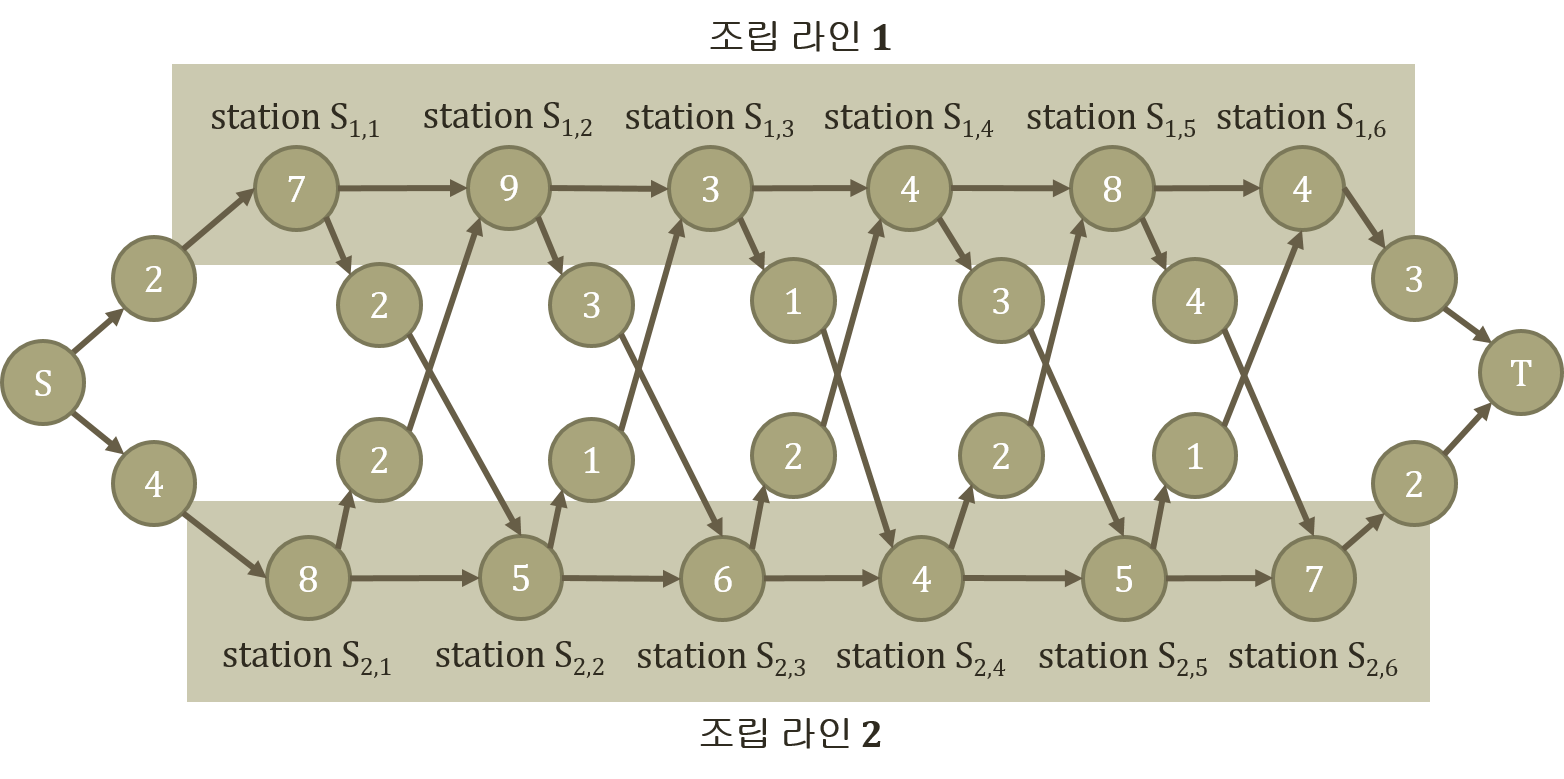
\includegraphics[scale=0.45]{fig9_13.png} 
\caption{조립 라인}
\label{fig:9-14}
\end{figure}

추적표를 사용하는 동적 계획법의 과정이 아직은 생소할 수 있으므로 여기서는 하나의 예시를 들어서 설명하고자 한다. 그림 \ref{fig:9-14}과 같은 자동차 생산 공장의 조립 라인이 있다. 자동차 조립은 맨 왼쪽의 $S$에서 시작해서 맨 오른쪽의 $T$에서 끝나며 중간에 모두 6가지의 공정이 필요하다. 각 공정에서는 조립 시간이 필요하며 같은 공정이라도 다른 조립 라인에서 한다면 소요 시간이 다를 수 있다. 각 공정은 첫 번째와 두 번째 조립 라인 중에서 어느 쪽에서 해도 괜찮지만 조립 라인을 갈아타는데도 정해진 만큼의 시간이 필요하다. 여기서 각 공정에 필요한 시간이나 조립 라인을 갈아타는데 드는 시간은 그림 \ref{fig:9-14}에 표시된 그대로이다.\\

문제는 최소한의 조립 시간을 찾으면서 실제로 공장을 운영할 수 있도록 각 공정별로 어떤 조립 라인에서 조립하는 것이 최적인가를 같이 요구하고 있다. 따라서 최소한의 조립 시간을 구하기 위한 메모이제이션 표 외에도 최적의 조립 라인을 구성하기 위한 역추적 작업에 필요한 추적표를 같이 구성해야 한다. \\

%슬라이드 21
\begin{figure}[ht] \centering 
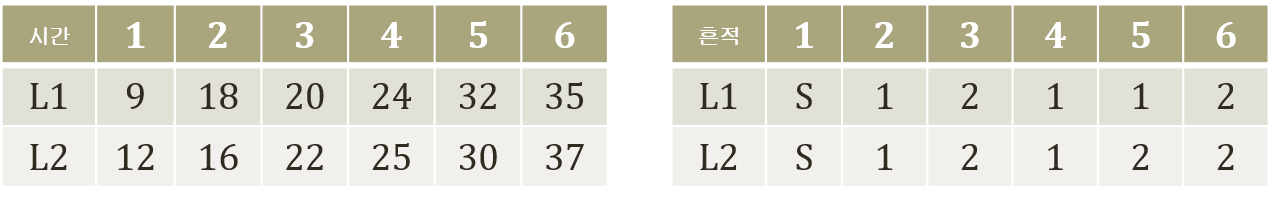
\includegraphics[scale=0.45]{fig9_14.png} 
\caption{메모이제이션 표와 추적표}
\label{fig:9-15}
\end{figure}

메모이제이션 표와 추적표는 다음과 같은 순서로 차례대로 채워나갈 수 있다. 먼저 시작 지점 $S$에서 $S_{1,1}$로 넘어가기 위해서는 한 가지 방법만이 있으며, 이동 시간인 2시간과 조립 시간인 7시간을 합해서 총 9시간이 걸린다. 따라서 메모이제이션 표와 추적표의 첫 번째 행, 첫 번째 열에는 각각 '9'와 'S'를 저장한다. 시작 지점 $S$에서 $S_{2,1}$로 넘어가는 데에도 한 가지 방법만이 있으며, 이동 시간인 4시간과 조립 시간인 8시간을 합해서 총 12시간이 걸린다. 따라서 메모이제이션 표와 추적표의 첫 번째 행, 두 번째 열에는 각각 '12'와 'S'를 저장한다. 이번에는 두 번째 공정으로 넘어가자. 첫 번째 공정으로부터 $S_{1,2}$로 넘어가기 위해서는 $S_{1,1}$에서 넘어오는 것과 $S_{2,1}$에서 넘어오는 것의 두 가지 방법이 있다. $S_{1,1}$과 $S_{1,2}$은 같은 라인에 있으므로 $S_{1,1}$에서 $S_{1,2}$으로 넘어가기 위해서는 $S_{1,1}$까지의 최소 시간인 9시간에서 조립 시간 9시간을 합쳐서 총 18시간이 걸린다. 한편, $S_{2,1}$과 $S_{1,2}$는 서로 다른 라인에 있으므로 $S_{2,1}$에서 $S_{1,2}$로 넘어가기 위해서는 $S_{2,1}$까지의 최소 시간인 12시간에서 이동 시간인 2시간과 조립 시간인 9시간을 합쳐서 총 23시간이 걸린다. 따라서 첫 번째 라인에서 넘어오는 것이 빠르므로 추적표의 두 번째 행, 첫 번째 열에는 '1'을 저장하고 그와 함께 메모이제이션 표에는 '18'을 저장한다. 이러한 과정을 $S_{2,2}$에 대해서 마찬가지로 진행할 수 있다. $S_{1,1}$에서 넘어오면 소요 시간이 최소 16시간이 걸리며 $S_{1,2}$에서 넘어오면 17시간이 걸린다. 따라서 메모이제이션 표와 추적표의 두 번째 행, 두 번째 열에는 각각 '16'과 '1'을 저장하면 된다. 이런 과정을 조립 라인별로, 공정별로 차례대로 진행한다면 여섯 번째 행까지 메모이제이션 표와 추적표를 채워 나갈 수 있다. \\ 

\begin{figure}[ht] \centering 
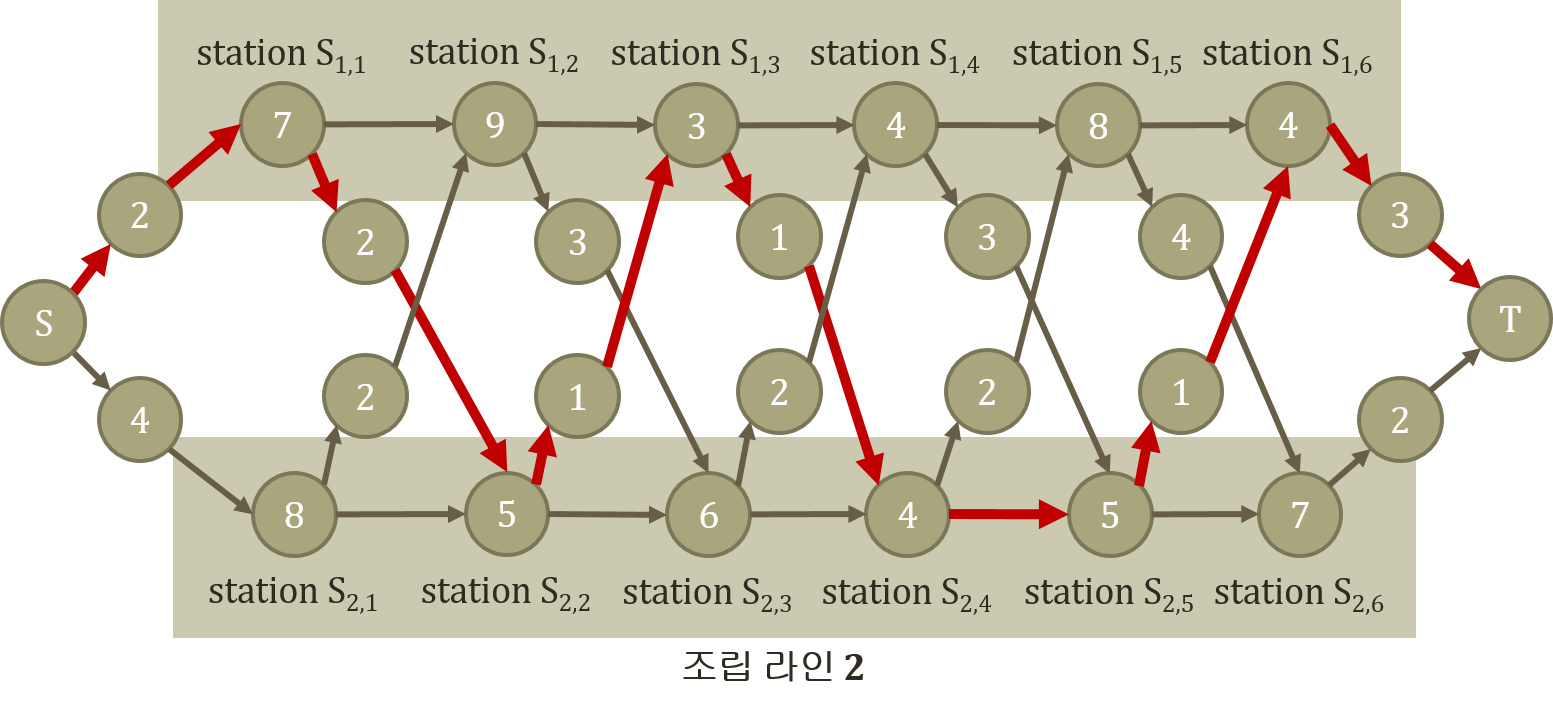
\includegraphics[scale=0.45]{fig9_15.png} 
\caption{추적표를 활용한 최적 경로 역추적}
\label{fig:9-16}
\end{figure}

이제 최소 시간과 최적 경로를 찾아보도록 하겠다. 그림 \ref{fig:9-15}의 메모이제이션 표에 따르면, $S_{1,6}$에 도달하는 최소 시간은 35시간이므로 $S_{1,6}$을 거쳐서 $T$에 도착하는 최소 시간은 여기에 3시간을 더한 38시간이다. 그리고 $S_{2,6}$에 도달하는 최소 시간은 37시간이므로 $S_{2,6}$을 거쳐서 $T$에 도착하는 최소 시간은 여기에 2시간을 더한 39시간이다. 양쪽을 비교하면 38시간이 더 작으므로 최소 시간은 38시간임을 알 수 있다. 그리고 최적 경로는 일단 $S_{1,6}$를 거쳐야 하는 것까지 확인하였으며, 나머지 경로는 추적표를 활용해서 역추적해나가야 한다. 먼저 추적표의 첫 번째 행, 여섯 번째 열을 보면 '2'라는 흔적이 남아 있다. 따라서 $S_{1,6}$으로 넘어가기 직전의 다섯 번째 공정은 두 번째 조립 라인인 $S_{2,5}$에서 이루어졌음을 알 수 있다. 다시 $S_{2,5}$에 해당하는 추적표의 두 번째 행, 다섯 번째 열을 확인하면 이번에는 '2'라는 흔적이 남아 있다. 따라서 $S_{2,5}$의 이전에는 $S_{2,4}$를 거쳤음을 알 수 있다. 같은 식으로 세 번째, 두 번째, 첫 번째 공정 또한 어느 라인에서 이루어졌는지를 역추적을 통해서 확인할 수 있으며, 그림 \ref{fig:9-16}처럼 이러한 과정으로 최소인 38시간이 걸리는 최적 경로를 구할 수 있다. \\

%슬라이드 22
지금까지 추적표를 사용하는 동적 계획법에 대해서 알아보고 예시를 통해서 이것을 이해할 수 있었다. 이제는 비터비 복호 알고리즘에서 추적표를 사용하는 동적 계획법이 어떻게 작동하는지를 알아보도록 하겠다. 알고리즘의 시작을 위해서는 초기값으로 $t=1$ 시점에서의 $V_{t}^{k}$ 값을 메모이제이션 표에 저장해야 한다. 여기서 $V_{t}^{k}$의 정의에 따르면 $V_{1}^{k}$는 확률값 $P(X_1, Z_1=z_{1}^{k})$와 같기 때문에 전향-후향 확률에서처럼 $b$와 $\pi$를 사용해서 다음과 같이 나타낼 수 있다. 
\begin{equation}
V_{1}^{k} = b_{k,X_1} pi_{k}
\label{eq:9-29}
\end{equation}
또한, 수식 (\ref{eq:9-28})의 결과를 가져와서 다음과 같은 재귀식을 세울 수 있으며, 이 때의 결과는 메모이제이션 표에 그대로 저장된다. 
\begin{equation}
V_{t}^{k} = b_{k,X_{t}} \textrm{max}_{i} a_{i,k} V_{t-1}^{k}
\label{eq:9-30}
\end{equation}
여기서 $V_{t}^{k}$ 값을 구하기 위한 $a_{i,k} V_{t-1}^{k}$를 최대로 만드는 $i$를 찾아서 추적표에 저장한다. 이런 식으로 추적표에 저장한 시간별, 직전 군집별 최적 군집은 동적 계획법 과정이 끝난 뒤의 최적해를 구하기 위한 역추적에 활용된다. 
\begin{equation}
U_{t}^{k} = \textrm{argmax}_{i} a_{i,k} V_{t-1}^{k}
\label{eq:9-31}
\end{equation}
이렇게 메모이제이션 표 $V$와 추적표 $U$를 동시에 구성하는 과정이 바로 비터비 복호 알고리즘의 동적 계획법 과정이다. 우리가 원하는 최대 확률값은 다음과 같이 메모이제이션 표의 $T$번째 열을 참조해서 구할 수 있다. 
\begin{equation}
\textrm{max}_{Z} P(X,Z) = \textrm{max}_{k} V_{T}^{k}
\label{eq:9-32}
\end{equation}
그리고 최적의 $Z$값은 $t=T$에서부터 시작해서 다음과 같이 하나씩 순서대로 찾아나갈 수 있다. 
\begin{equation}
Z_{T}^{*} = \textrm{argmax}_{k} V_{T}^{k}, \ \ Z_{t-1}^{*} = U_{t}^{Z_{t}^{*}}, t=T,\cdots,2
\label{eq:9-33}
\end{equation} 

지금까지가 비터비 복호 알고리즘의 전체 과정으로서 이론적으로는 완벽하다고 할 수 있다. 하지만 이것을 현실에서 구현하다 보면 언더플로우(Underflow) 문제가 생길 수 있다. 앞서 예시에서는 그래프 모델에서 고려하는 시간의 개수가 세 개 뿐이였지만 현실에서는 시간의 개수가 수백에서 수천 개 이상이 될 수 있다. 이것은 계산 과정에서 수천 개 이상의 확률값을 곱해야 한다는 것과 같다. 그러나 컴퓨터는 수많은 확률값을 곱하면서 너무나도 작아진 값을 0으로 취급할 수 있으며 이러한 과정에서 언더플로우 문제가 발생한다. 이러한 언더플로우 문제를 해결하기 위해서 계산 과정에서 로그 함수를 사용하는 방법이 있다. 로그 함수를 사용한다면 컴퓨터는 원래의 확률값 대신 그것의 지수를 저장하기 때문에 저장할 값이 0에 가까워지는 것을 막을 수 있다. 실제 우리가 사용하는 기계 학습 라이브러리에서도 로그 함수를 사용해서 확률값을 계산할 수 있도록 구현되어 있다. \\

%-----------------------------------------------------------------
\subsection{바움-웰치 알고리즘}
%-----------------------------------------------------------------

%슬라이드 23, 24
앞에서 다룬 전향-후향 확률 계산과 비터비 복호 알고리즘은 파라미터 $\pi$, $a$, $b$가 사전 정보로 주어진 상태에서 은닉 마르코프 모델의 확률을 계산하였다. 이번에는 파라미터 $\pi$, $a$, $b$의 값을 모르면서 관찰 변수인 $X$만 주어진 상황에서의 문제인 학습 질문를 다루고자 한다. 학습 질문에서는 군집화의 중심에 대한 어떠한 정보도 제공하지 않는다. 따라서 우리는 이번에야말로 시계열 데이터만이 주어진 상황에서 군집화를 어떤 식으로 진행하는지를 이해할 수 있다. 학습 질문을 다룰 수 있는 대표적인 알고리즘으로는 바움-웰치 알고리즘이 있으며 이번 장에서 자세히 알아볼 것이다. \\

바움-웰치 알고리즘(Baum-Welch Algorithm)은 은닉 마르코프 모델의 파라미터가 주어지지 않았을 때 파라미터의 값과 은닉 변수의 값을 동시에 구할 수 있도록 하는 특수한 형태의 EM 알고리즘을 말한다. 일반적인 EM 알고리즘과 마찬가지로 여기에도 기댓값 과정과 최대화 과정이 있으며 바움-웰치 알고리즘은 이 두 과정을 번갈아 가면서 실행한다. 최대화 과정에서는 군집의 형태를 결정하는 파라미터 $pi$, $a$, $b$의 값을 결정한다. 그리고 기댓값 과정에서는 최대화 과정에서 구한 파라미터 $\pi$, $a$, $b$를 바탕으로 해서 시계열 데이터 포인트가 시간별로 어떤 군집에 속하는지를 최적인 은닉 변수 $Z$의 값을 알아낸다. \\

%슬라이드 25
은닉 마르코프 모델을 위한 EM 알고리즘을 시작하기 위해서는 먼저 $\pi$, $a$, $b$의 초기값인 $\pi^{0}$, $a^{0}$, $b^{0}$를 임의로 정해주어야 한다. 이것은 아직 어떠한 과정도 거치지 않아 적절한 $\pi$, $a$, $b$를 계산할 수 있는 정보가 $X$ 외에는 주어져 있지 않기 때문이다. 기댓값 과정에서는 기댓값 과정을 $s$번 반복한 결과인 파라미터 값을 받아서 $Z$의 $s+1$번째 확률 분포 함수 $q^{s+1}$을 찾는다. 여기서 첫 번째 함수인 $q^1$은 파라미터의 초기값을 바탕으로 정할 수 밖에 없다. 그러나 두 번째 기댓값 과정에서부터는 직전의 최대화 과정에서 구한 파라미터인 $\pi^{s}$, $a^{s}$, $b^{s}$가 있으므로 이것을 바탕으로 $Z$의 확률 분포 함수 $q^{s+1}$을 정할 수 있다.  \\

기댓값 과정을 진행한 직후에는 최대화 과정을 통해서 우리가 이미 알고 있는 관찰 변수 $X$와, $s+1$번째 최대화 과정을 거쳐서 나온 $Z$의 확률 분포인 $q^{s+1}$을 바탕으로 가장 적절한 $\pi$, $a$, $b$의 값인 $\pi^{s+1}$, $a^{s+1}$, $b^{s+1}$을 구해야 한다. 여기서 가장 적절한 $\pi$, $a$, $b$란 로그 우도 $Q(\pi, a, b, q^{s})$의 값을 최대로 만드는 $\pi$, $a$, $b$을 말한다. 여기까지는 원래의 EM 알고리즘과 같으나 여기서는 $\pi$, $a$, $b$가 확률에 관한 파라미터이므로 이들 벡터를 구성하는 숫자들의 합이 정확히 1이여야 한다는 조건을 추가로 생각해야 한다. 이러한 최대화 과정을 하나의 식으로 나타내면 다음과 같이 나온다.
\begin{eqnarray}
(\pi^{s+1}, a^{s+1}, b^{s+1}) & = & \textrm{argmax}_{\pi, a, b} Q(\pi, a, b, q^{s+1}) \nonumber \\
& = & \textrm{argmax}_{\pi, a, b} E_{q^{s+1}(Z)} \textrm{ln} P(X, Z|\pi, a, b) + H(q^{s+1}) \nonumber \\ 
& = & \textrm{argmax}_{\pi, a, b} E_{q^{s+1}(Z)} \textrm{ln} P(X, Z|\pi, a, b) \label{eq:9-34}
\end{eqnarray}

그러나 수식 (\ref{eq:9-34})는 아직까지는 무엇을 최대로 만들어야 하는지를 제시하고 있을 뿐이다. 이 식을 전개해서 우리가 무엇을 해야하는지를 확실히 해 보자. $\pi$, $a$, $b$가 주어진 상황에서 $X,Z$의 결합 확률은 다음과 같다. 
\begin{equation}
P(X,Z|\pi,a,b) = \pi_{Z_1} \prod_{t=2}^{T} a_{Z_{t-1}, Z_{t}} \cdot \prod_{t=1}^{T} b_{Z_{t}, X_{t}} 
\label{eq:9-35}
\end{equation} 
이것은 은닉 마르코프 모델의 결합 확률을 분해한 것이며 이것을 수식 (\ref{eq:9-34})에 대입하기 위해서는 다음과 같이 $P(X,Z|\pi,a,b)$에 대해서 로그를 취해야 한다.
\begin{equation}
\mathrm{ln} P(X,Z|\pi,a,b) = \mathrm{ln} \pi_{Z_1} + \sum_{t=2}^{T} \mathrm{ln} a_{Z_{t-1}, Z_{t}} + \sum_{t=1}^{T} \mathrm{ln} b_{Z_{t}, X_{t}} 
\label{eq:9-36}
\end{equation} 
한편, 기댓값의 정의를 활용해서 수식 (\ref{eq:9-34})의 $E_{q^{s+1}(Z)} \textrm{ln} P(X, Z|\pi, a, b)$를 다음과 같이 나타낼 수 있다. 
\begin{eqnarray}
E_{q^{s+1}(Z)} \textrm{ln} P(X, Z|\pi, a, b) & = & \sum_{Z} q^{s+1}(Z) \mathrm{ln} P(X,Z|\pi,a,b) \nonumber \\
& = & \sum_{Z} P(Z|X,\pi^{s}, a^{s}, b^{s}) \mathrm{ln} P(X,Z|\pi,a,b) \label{eq:9-37}
\end{eqnarray} 
%슬라이드 26 
그리고 여기에 수식 (\ref{eq:9-36})을 대입해서 우리가 최대로 만들어야 할 $Q$를 다음과 같이 나타낼 수 있다.
\begin{equation}
\sum_{Z} P(Z|X,\pi^{s}, a^{s}, b^{s}) \{\mathrm{ln} \pi_{Z_1} + \sum_{t=2}^{T} \mathrm{ln} a_{Z_{t-1}, Z_{t}} + \sum_{t=1}^{T} \mathrm{ln} b_{Z_{t}, X_{t}}\}
\label{eq:9-38}
\end{equation} 
  
이제 수식 (\ref{eq:9-38})을 최적으로 만드는 $\pi$, $a$, $b$를 구하는 방법에 대해서 생각해 보도록 하겠다. 앞에서도 설명했다시피 여기에는 이들 벡터는 구성 성분의 합이 정확히 1이여야 한다는 조건이 추가로 붙어 있다. 따라서 수식 (\ref{eq:9-38})의 최적화를 위해서 chapter 5와 chapter 8에서 사용했던 라그랑지 방법을 다시 가져와서 적용해야 한다. $X$와 $Z$가 모두 다항 분포라는 것을 생각하면 라그랑지 함수를 다음과 같이 구성할 수 있다.
\begin{equation}
L(\pi, a, b, q^{s+1}) = Q(\pi, a, b, q^{s+1}) - \lambda_{\pi} (\sum_{i=1}^{K} \pi_i - 1) - \sum_{i=1}^{K} \lambda_{a_i} ( \sum_{j=1}^{K} a_{i,j} - 1) - \sum_{i=1}^{K} \lambda_{b_i} ( \sum_{j=1}^{M} b_{i,j} - 1)
\label{eq:9-39}
\end{equation} 
여기서 $\lambda_{\pi}$, $\lambda_{a_i}$, $\lambda_{b_i}$는 각각의 등호 조건식에 붙는 라그랑지 승수이다. 여기서 $\pi$의 값을 구하기 위해서는 $L(\pi, a, b, q^{s+1})$을 각 $\pi_i$에 대해서 편미분을 하고, 각각이 모두 0과 같다는 방정식을 세워야 한다. 그리고 $\pi$에 대한 조건식인 $\sum_{i=1}^{K} \pi_i = 1$을 함께 놓고 방정식을 풀어서 각 $\pi_{i}$의 값을 구해야 한다. 이런 식으로 계산을 하면 $\pi_{i}$의 값은 다음과 같이 나온다. 
\begin{equation}
\pi_{i}^{s+1} = \frac{P(Z_1^{i}=1 | X, \pi^{s}, a^{s}, b^{s})}{\sum_{k=1}^{K} P(Z_1^{k}=1 | X, \pi^{s}, a^{s}, b^{s})}
\label{eq:9-43}
\end{equation} 
같은 식으로 $a_{i,j}^{s+1}$, $b_{i,j}^{s+1}$의 값 또한 구할 수 있다. 
\begin{equation}
a_{i,j}^{s+1} = \frac{\sum_{t=2}^{T} P(Z_{t-1}^{i}=1, Z_{t}^{i}=1 | X, \pi^{s}, a^{s}, b^{s})}{\sum_{t=2}^{T} P(Z_{t-1}^{i}=1 | X, \pi^{s}, a^{s}, b^{s})}
\label{eq:9-44}
\end{equation} 
\begin{equation}
b_{i,j}^{s+1} = \frac{\sum_{t=1}^{T} P(Z_{t}^{i}=1 | X, \pi^{s}, a^{s}, b^{s}) \delta(X_{t}^{j}=1)}{\sum_{t=1}^{T} P(Z_{t}^{i}=1 | X, \pi^{s}, a^{s}, b^{s})}
\label{eq:9-45}
\end{equation} 
여기서 $\delta(X_{t}^{j}=1)$는 $X_{t}$의 $j$번째 항목이 1일 때만 1이고 그 외에는 0인 함수이다. \\ 
%이렇게 은닉 마르코프 모델을 위한 EM 알고리즘의 최대화 과정에서 파라미터에 \\

%슬라이드 27
지금까지의 설명을 바탕으로 이제는 바움-웰치 알고리즘을 어떻게 적용할지 구체적으로 설명할 수 있다. 바움-웰치 알고리즘을 시작하기 위해서는 먼저 파라미터의 초기값인 $\pi^{0}$, $a^{0}$, $b^{0}$를 임의로 정해주어야 한다. 그리고 나서는 기댓값 과정과 최대화 과정을 번갈아 가면서 시행하면 된다. 기댓값 과정에서는 맨 처음에 정한 초기값이나 최대화 과정에서 구한 $\pi^{s}$, $a^{s}$, $b^{s}$를 활용해서 각각의 $t$와 $k$에 대해서 전향, 후향 확률값인 $\alpha_{t}^{k}$, $\beta_{t}^{k}$를 구한다. 그리고 이것을 바탕으로 $P(Z_{t}^{i}=z_{t}^{i},X)=\alpha_{t}^{k}\beta_{t}^{k}$와 $P(X)=\sum_{k} \alpha_{t}^{k}$를 구한다. 최대화 과정에서는 $\pi_{i}^{s+1}$, $a_{i,j}^{s+1}$, $b_{i,j}^{s+1}$의 값을 기댓값 과정에서 구한 확률값들을 바탕으로 계산한다. 여기서 계산은 수식 (\ref{eq:9-43}), (\ref{eq:9-44}), (\ref{eq:9-45})를 바탕으로 이루어지며 이들을 구하기 위해서는 $P(Z_{t}^{i}=z_{t}^{i},X)$가 $P(Z_{t}^{i}=z_{t}^{i}|X)P(X)$와 같다는 사실과 $P(Z_{t}^{i}=z_{t}^{i}, Z_{t-1}^{i}=z_{t-1}^{i} | X)$가 $a_{Z_{t-1},Z{t}}^{s} P(Z_{t-1}^{i}=z_{t-1}^{i}| X)$와 같다는 사실을 이용할 수 있다.  


\end{document}
